\section{Trigonometria no Triângulo Retângulo}

\begin{definition}
\label{def:seno-cosseno-triangulo-retangulo}
Em um triângulo retânglulo $ABC$, como na Imagem~\ref{fig:triangulo-retangulo}, definem-se o
\textdef{cosseno} ($\cos$) e o \textdef{seno} ($\sen$) dos ângulos agudos do
triângulo:
%
$$\cos \widehat B = \frac c a = \frac {\text{cateto
adjacente}}{\text{hipotenusa}}, \ \ \ \ \sen \widehat B = \frac b a = \frac
{\text{cateto oposto}}{\text{hipotenusa}},$$
$$\cos \widehat C = \frac b a \ \ \ \ \text{e} \ \ \ \ \sen \widehat
C = \frac c a.$$    
%
\begin{figure}[H]
\centering
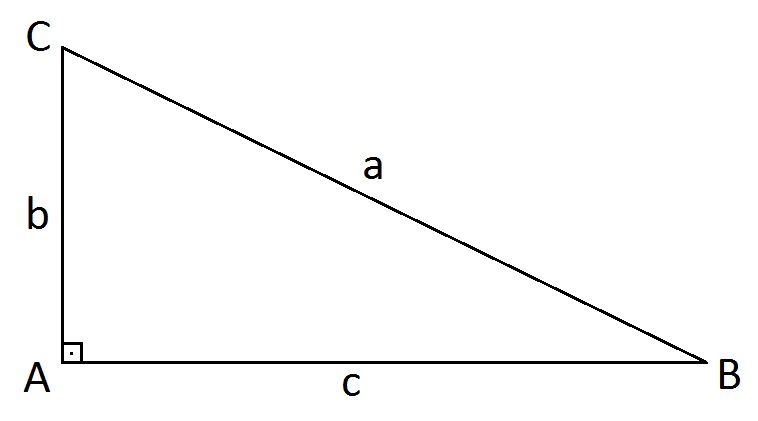
\includegraphics[scale=0.4]{\imgdirfromsection/triangret.jpg}
\caption{Triângulo retângulo qualquer.}
\label{fig:triangulo-retangulo}
\end{figure}
\end{definition}

\begin{remark}
As relações definidas como o foram na Definição~\ref{def:seno-cosseno-triangulo-retangulo} são únicas para cada ângulo em
decorrência da proporcionalidade dos lados de triângulos
semelhantes. Portanto, calculam-se o seno e o cosseno de um ângulo
independentemente do triângulo retângulo que o contém.
\end{remark}

\begin{proposition}
Os seguintes valem:
\begin{itemize}
    \item O cosseno de um ângulo agudo é igual ao seno do seu
    complementar e vice-versa (daí surgiu o termo ``cosseno'': seno do complemento);
    \item O seno e o cosseno são números compreendidos entre 0 e 1, uma vez que são razões entre um cateto 
    e a hipotenusa de um triângulo retângulo.
\end{itemize}
\end{proposition}

\begin{proof}
    Sejam $\widehat B$ um ângulo agudo e $\triangle ABC$ um triângulo tal que um de seus ângulos mede $\widehat B$.
    A situação é ilustrada na Imagem~\ref{img:triangulo-retangulo-generico}.
    %
    \begin{figure}[H]
        \centering
        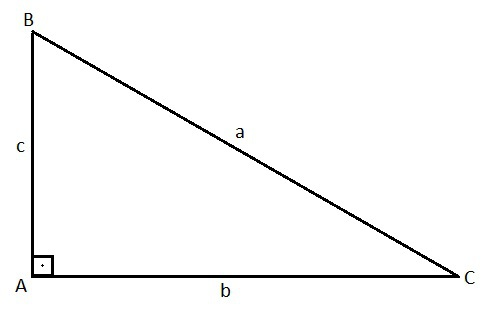
\includegraphics[scale=0.65]{\imgdirfromsection/triangulo-retangulo-generico.jpg}
        \caption{Triângulo retângulo qualquer.}
        \label{img:triangulo-retangulo-generico}
    \end{figure}
    %
    Temos que $\widehat A + \widehat B  + \widehat C = 180\degree$, ou seja, $\widehat B  + \widehat C = 90\degree$.
    Logo, $\widehat B$ e $\widehat C$ são complementares. Segue que:
    %
    $$\cos \widehat B = \frac c a = \sen \widehat C.$$ Portanto, o cosseno de um ângulo agudo é igual ao seno do seu complementar,
    e vice-versa. Ademais, pelo fato de a hipotenusa ser o maior dos lados de um triângulo retângulo, já que é oposta ao 
    maior dos ângulos desse triângulo, segue que qualquer razão de um cateto pela hipotenusa será um número entre 0 e 1.
\end{proof}

\begin{proposition}[Relação Fundamental da Trigonometria]
Seja $\widehat B$ um dos ângulos agudos de um triângulo retângulo
cuja hipotenusa mede $a$ e os catetos, $b$ e $c$. Então:
$$\sen^2 \widehat B + \cos^2 \widehat B = 1.$$
\end{proposition}

\begin{proof}
    Seja $\triangle ABC$ um triângulo retânglulo tal que $\widehat B$ é um de seus ângulos agudos. A situação é 
    mostrada na Imagem~\ref{img:prova-relacao-fundamental-trigonometria}.
    %
    \begin{figure}[H]
        \centering
        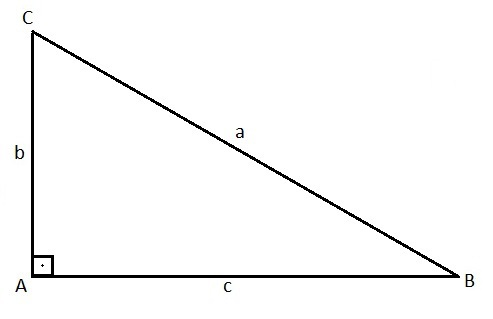
\includegraphics[scale=0.65]{\imgdirfromsection/triangulo-retangulo-generico2.jpg}
        \caption{Triângulo retângulo qualquer.}
        \label{img:prova-relacao-fundamental-trigonometria}
    \end{figure}
    %
    Do Teorema de Pitágoras, temos:
    %
    \begin{align*}
        b^2 + c^2 = a^2 &\iff \frac{b^2}{a^2} + \frac{c^2}{a^2} = 1 \\ &\iff \prn{\frac b a}^2 + \prn{\frac c a}^2 = 1 \\ 
        &\iff \sen^2 \widehat B  +  \cos^2 \widehat B= 1.
    \end{align*}
\end{proof}

\begin{onlineact}
    \khan{https://pt.khanacademy.org/math/trigonometry/trigonometry-right-triangles/intro-to-the-trig-ratios/e/trigonometry_1}
    {Razões Trigonométricas em Triângulos
Retângulos}.
\end{onlineact}

\begin{onlineact}
    \khan{https://pt.khanacademy.org/math/trigonometry/trigonometry-right-triangles/trig-solve-for-a-side/e/trigonometry_2}
    {Como Calcular a Medida de um Lado em Triângulos Retângulos}.
\end{onlineact}